% Generated inclusion template for the NSSR qualitative figures.
% Adjust the relative graphics path to match the manuscript directory.

\begin{figure*}[t]
\centering
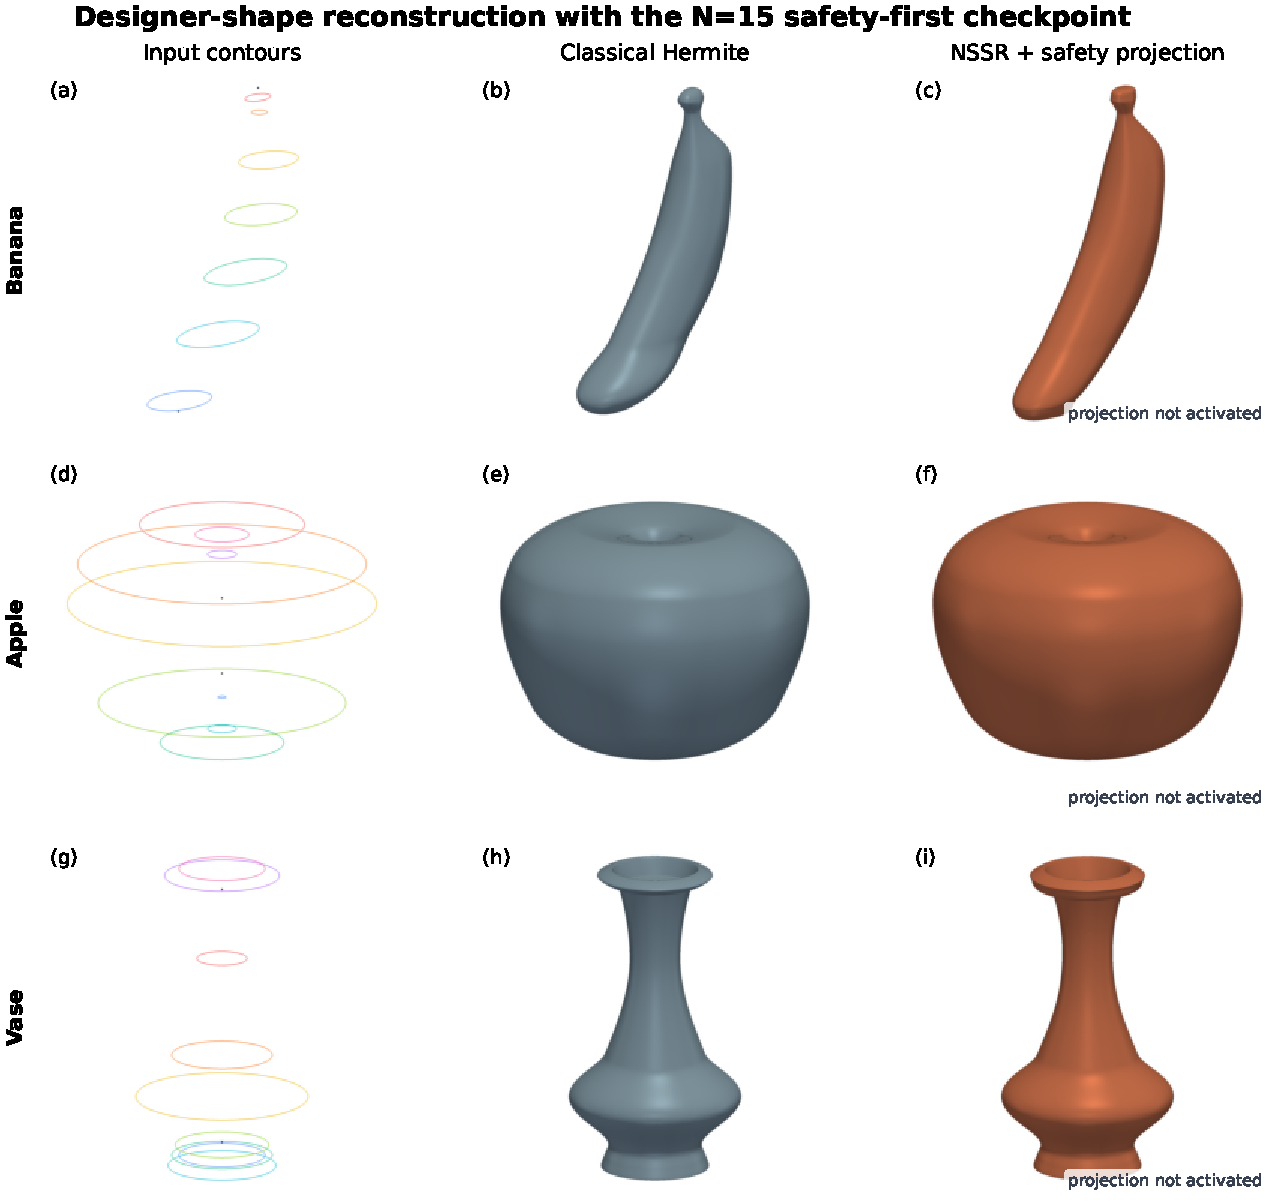
\includegraphics[width=\textwidth]{figure_designer_comparison_N15.pdf}
\caption{Designer-shape reconstructions using the synthetic-trained,
safety-first $N=15$ checkpoint.  Each row shows the ordered input contours,
the zero-correction classical Hermite surface, and the final NSSR surface
after the shared sampled-safety projection plus the designer-specific axis
clearance check.  The computational surfaces use $m=128$ unique periodic
circumferential samples; seam duplication is used for display only.}
\label{fig:nssr_designer_qualitative}
\end{figure*}

\begin{figure*}[t]
\centering
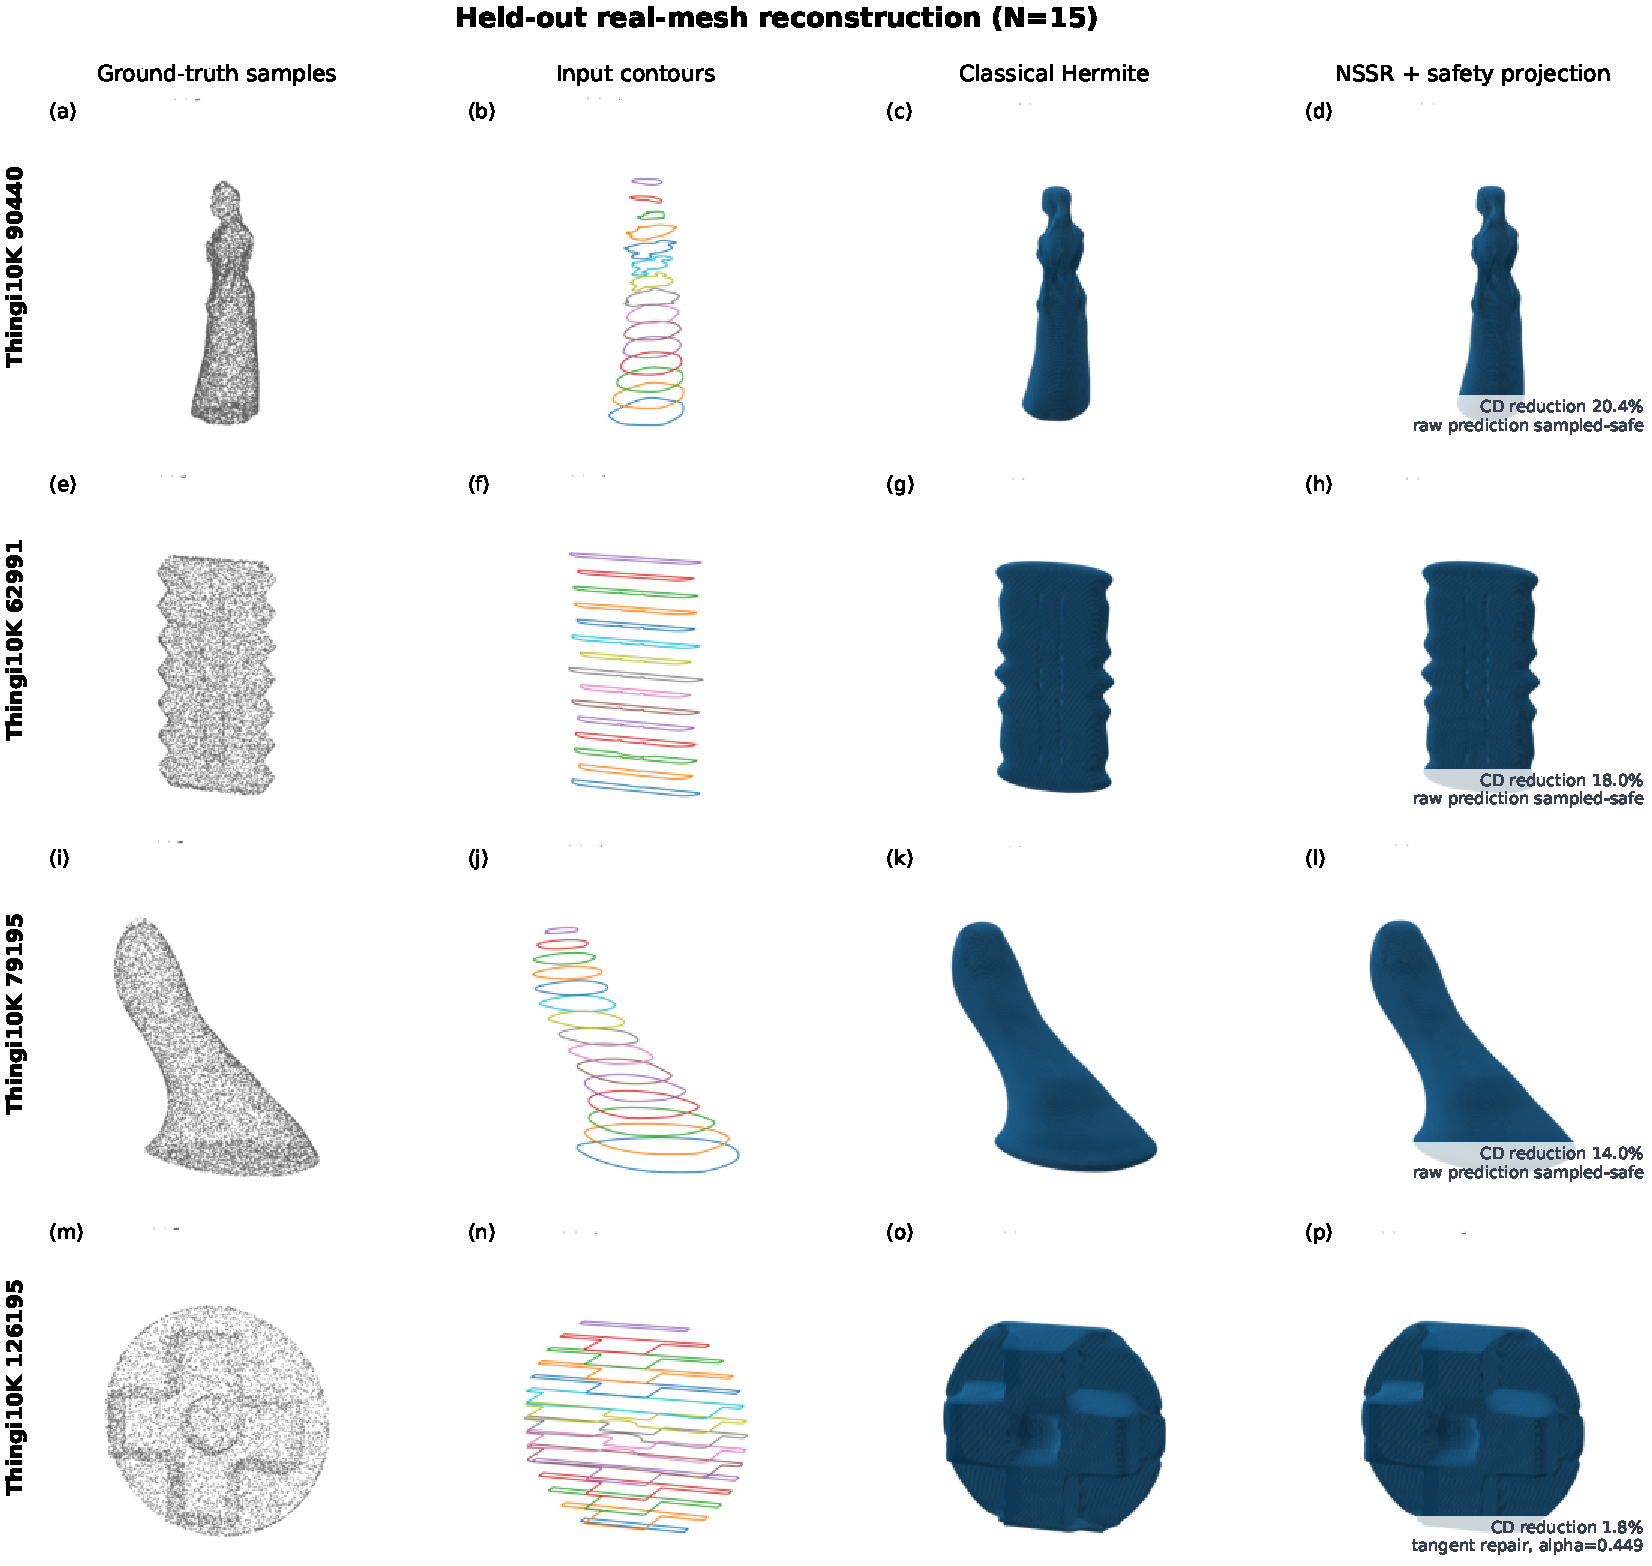
\includegraphics[width=\textwidth]{figure_real_comparison_N15.pdf}
\caption{Representative held-out real-mesh reconstructions for the
real-trained, safety-first $N=15$ checkpoint.  Columns show ground-truth
samples, the sparse input contour stack, the classical Hermite surface, and
the final post-projection NSSR surface.  The examples were selected to cover
distinct silhouettes and accuracy gains and include a case requiring
tangent-stage repair; selection was not used for any aggregate metric.}
\label{fig:nssr_real_qualitative}
\end{figure*}

\begin{figure*}[t]
\centering
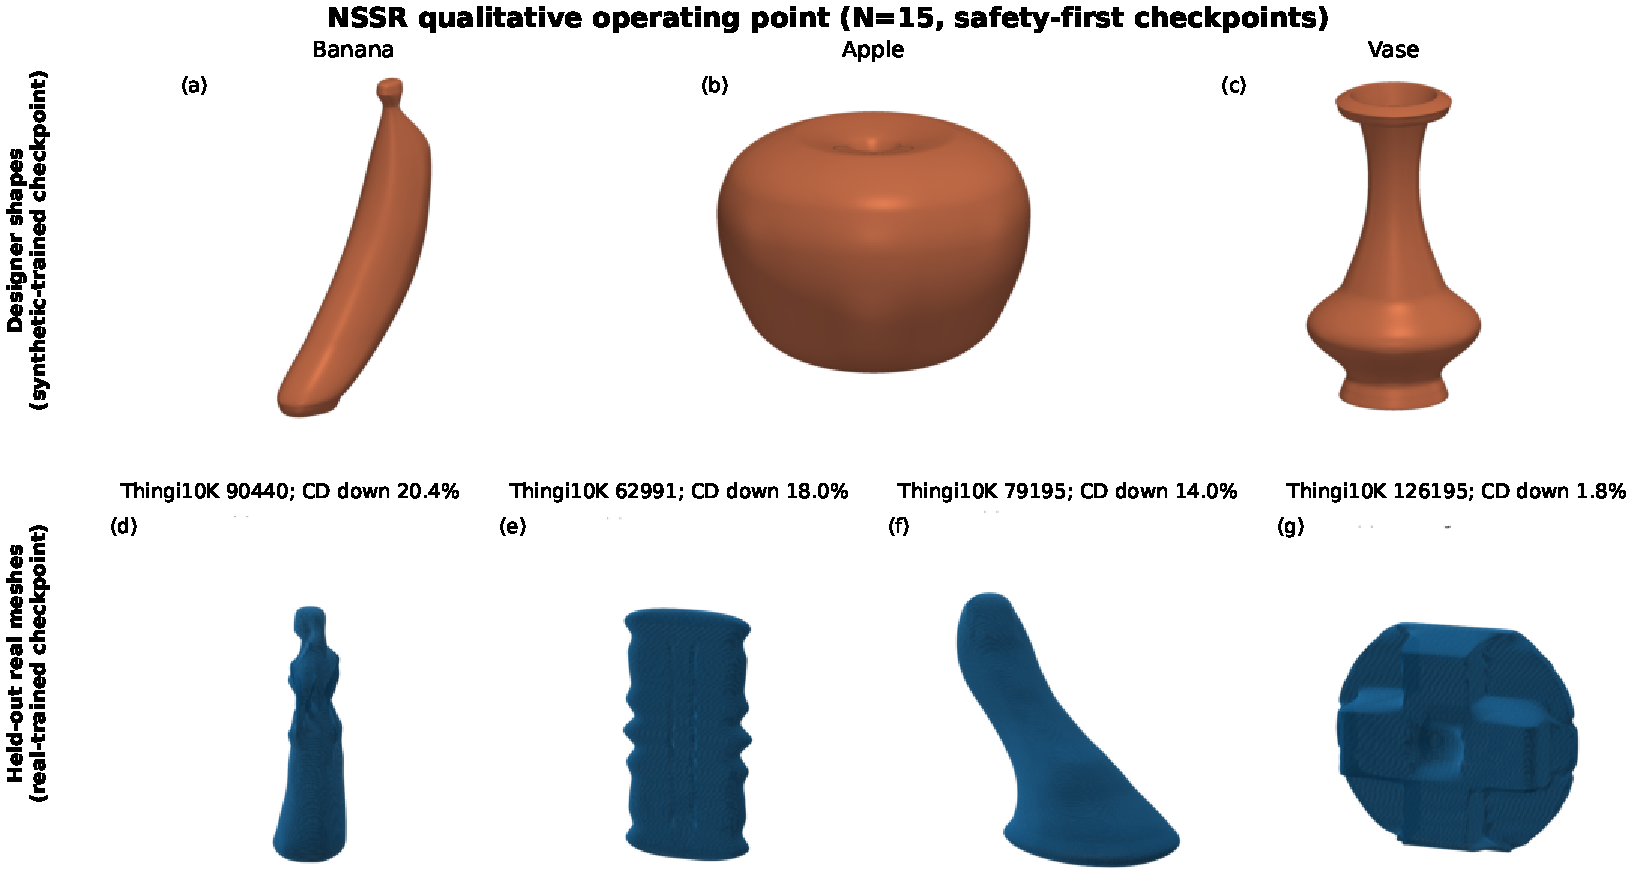
\includegraphics[width=\textwidth]{figure_qualitative_combined_N15.pdf}
\caption{Compact qualitative gallery at the strongest slice-count operating
point, $N=15$.  The upper row uses the synthetic-trained checkpoint on the
three hand-designed contour stacks; the lower row uses the real-trained
checkpoint on held-out real meshes.  Every displayed NSSR output is the final
state returned by the sampled-safety projection.}
\label{fig:nssr_qualitative_gallery}
\end{figure*}
